\section{\crdb and \crdbxx}\label{sec:crdb}
This section presents the design, implementation, and evaluation of Cockroachdb (for short, CRDB) and CRDB-RLS. We show that RLS has the potential to evolve the consistency model of existing databases (i.e., providing tighter and stronger consistency guarantees) without sacrificing performance. 

\subsection{Protocols and Implementations}

\noindent\textbf{CRDB Background.} CRDB~\cite{taft2020cockroachdb} is an open-source production-grade database system that began as an external Spanner clone. Like Spanner, CRDB aims to build a resilient geo-distributed SQL Database with serializable ACID transactions.

Overall, \crdb provides single-key linearizability (i.e., no stale reads for each key) by supporting multi-version timestamp ordering (MVTO). The transaction manager nodes in CRDB are the special nodes for interacting with clients, assigning timestamps to transactions, and driving transaction coordination. CRDB assumes a maximum clock offset among transaction managers (i.e., using $500ms$ by default), which is critical to its correctness.

\crdb's consistency model (i.e., single-key linearizability) is strictly weaker than \xxcons as \crdb ensures only a subset of \xxcons's guarantees: \crdb does not preserve the real-time ordering for any pair of non-conflicting transactions, while RLS provides real-time order among IRTs in the same region. We refer readers to \chref{sec:rls:compare} for detailed comparisons between RLS and Single-Key Linearizability (SKL). 

\newcommand\mycommfont[1]{\footnotesize\sffamily\textcolor{red}{#1}}
\SetCommentSty{mycommfont}
\SetKwProg{Fn}{function}{:}{}

\SetKwFunction{FMax}{max}
\SetKwFunction{FNow}{now}
\SetKwFunction{Coordcr}{CRDB-RLS Coordinator}
\SetKwFunction{FGetFinTs}{GetFinishedTs}
\SetKwFunction{FVerifyReads}{VerifyReads}
\SetKwFunction{Leader}{GetShardLeader}
\SetKwFunction{FSend}{send}
\SetKwFunction{FKeyLeader}{keyLeader}

\SetKwData{InFlightOps}{inflightOps}
\SetKwData{TouchedR}{touchedRegions}
\SetKwData{TxnTs}{txnTS}
\SetKwData{DOp}{op}
\SetKwData{DRegion}{r}
\SetKwData{DResp}{resp}

\begin{algorithm}[t]
    \setstretch{1}
    \small
    % \LeftComment{Execute the transaction commands, which triggers the events:}
    \Fn{\Coordcr}{
      \InFlightOps $\gets \emptyset$   \Comment{Ongoing operations.} \\
      \TouchedR $\gets \emptyset$  \Comment{Regions involved in the transaction.} \\
      \TxnTs $\gets$ \FNow{}   \Comment{Timestamp of the transaction.} \\

      \For{\DOp $\gets$ KV operation received from SQL layer}{
        \uIf{\DOp.commit}{
          \DOp.deps $\gets$ \InFlightOps \\
          \FSend $\langle \texttt{commit}, \TxnTs \rangle$ to transaction managers \\
          wait for all \texttt{ACK}s \\
        }
        \Else(){
          % \tcp{New in \crdbxx}
          \tikzmk{A}
          \DRegion $\gets$ \DOp.key.region \\
          \If{$\DRegion \notin \TouchedR$}{
            \TxnTs $\gets$ \FMax{\TxnTs, \FGetFinTs{\DRegion}} \\
            \FVerifyReads{\TxnTs} \\
            \TouchedR $\gets$ \TouchedR $\cup$ \{\DRegion\} \\
          }
          \tikzmk{B} \boxit{blue}
          % \tcp{Original algorithm of \crdb.}
          \DOp.deps $\gets$ $\{ x \in$ \InFlightOps $| x.key = \DOp.key \}$ \\
          \InFlightOps  $\gets$ (\InFlightOps - \DOp.deps) $\cup$ $\{ \DOp \}$
     \DResp $\gets$ \FSend{\DOp, \FKeyLeader{\DOp.key}} \\
          \TxnTs $\gets$ \FMax{\TxnTs, \FGetFinTs{\DRegion}} \\
          \FVerifyReads{\TxnTs} \\
        }
      }    
    }
    \caption{Algorithm of \crdbxx Coordinator}\label{algo4}
\end{algorithm}

\crdb makes such a design choice because, without the two-layered design of \xxcons, the developers could only choose the consistency model between extreme ends of the spectrum: either enforcing all real-time constraints among non-conflicting transactions (i.e., strict serializability) or enforcing none of them. Since implementing strict serializability across regions can easily overwhelm the benefits of data locality and severely impact performance, \crdb has chosen the latter approach. Consequentially, \crdb cannot even guarantee the causal relation of two transactions from the same client when they access different keys in the same region.

CRDB performs its reads and writes at its commit timestamp, relying heavily on multi-version concurrency control (MVCC) to process concurrent requests. When a transaction conflicts with other transactions, CRDB adjusts the transaction's commit timestamp to ensure single-key linearizability. Since conflict detection is only conducted in the critical granularity, CRDB does not provide any consistency guarantees when two transactions do not conflict with each other. 


\xxcons provides a better design point in the spectrum. To demonstrate the pros and cons of \xxcons, we re-design the protocol of \crdb by incorporating multi-region semantics into the conflict detection progress, resulting in \crdbxx. 

\noindent\textbf{CRDB-RLS.}  
\algo{algo4} illustrates the pseudocode of CRDB-RLS, with multi-region semantics highlighted in blue. To achieve \xxcons, for any two transactions $T_1$ and $T_2$ that access overlapped regions, if $T_1$ have finished, \crdbxx ensures that $T_2$'s timestamp is larger than $T_1$'s.  \crdb achieves this by comparing with $T_1$'s write timestamp when $T_2$'s read arrives. Specifically, if $T_2.ts > T_1.ts$, $T_2$ must see $T_1$'s write; otherwise, if $T_2.ts < T_1.ts$, $T_1$ may still finish before $T_2$ starts due to clock skewness, but the skewness should have an assumed bound (i.e., $500ms$ in the codebase of CRDB). Consequentially, if $T_1.ts - T_2.ts < bound$, \crdb cannot determine the order between $T_1$ and $T_2$. In such a case, CRDB enforces $T_2$ to abort and then lets it retry automatically. 

\begin{figure}[t]
	\centering
	\subfloat[\footnotesize Throughput.]{
	   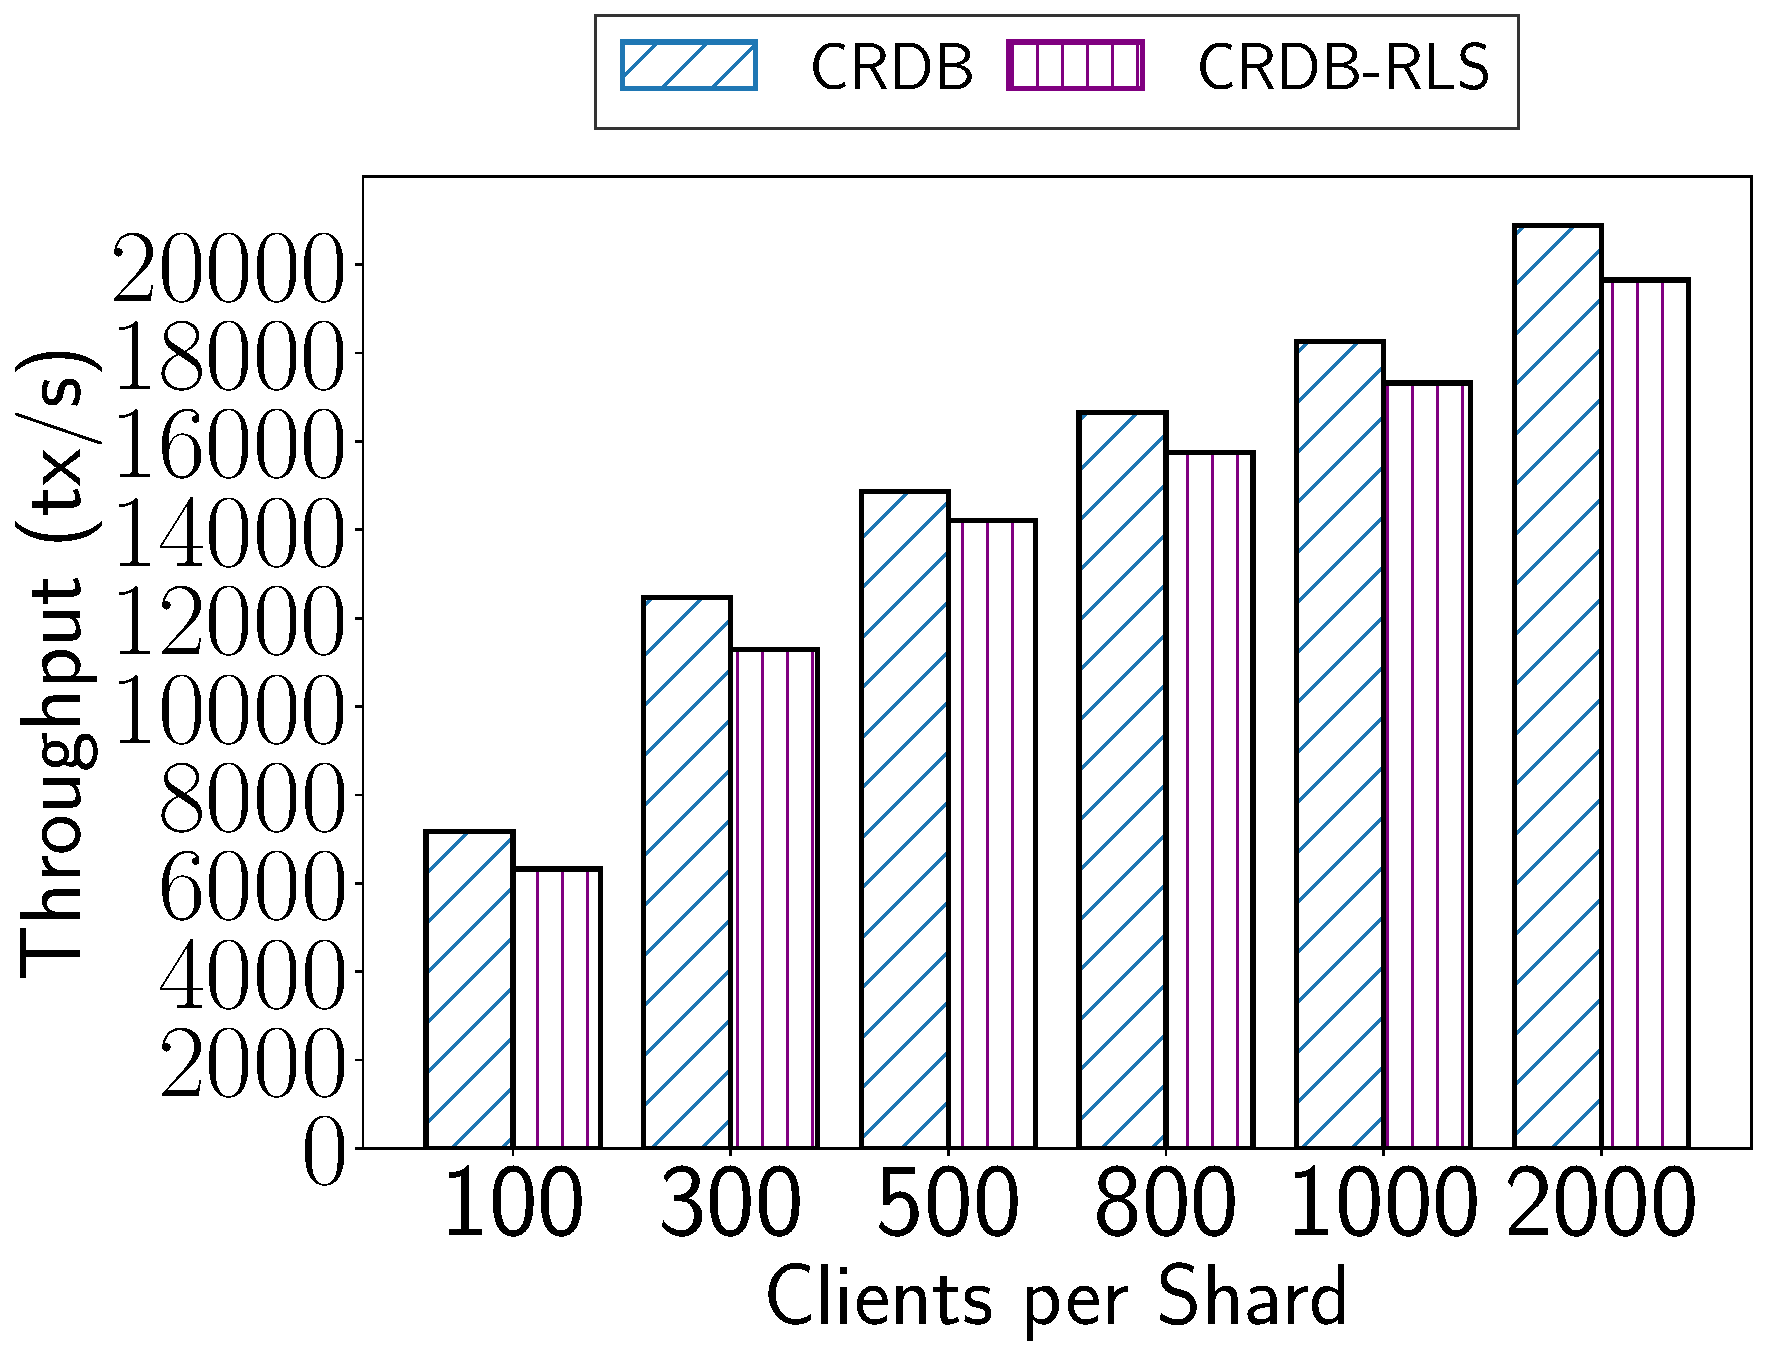
\includegraphics[width=0.49\columnwidth]{eval-figs/crdb-client--tput-kv.pdf}
	   \label{fig:eval:kv:throughput}
	}
	\subfloat[\footnotesize Overview.]{
		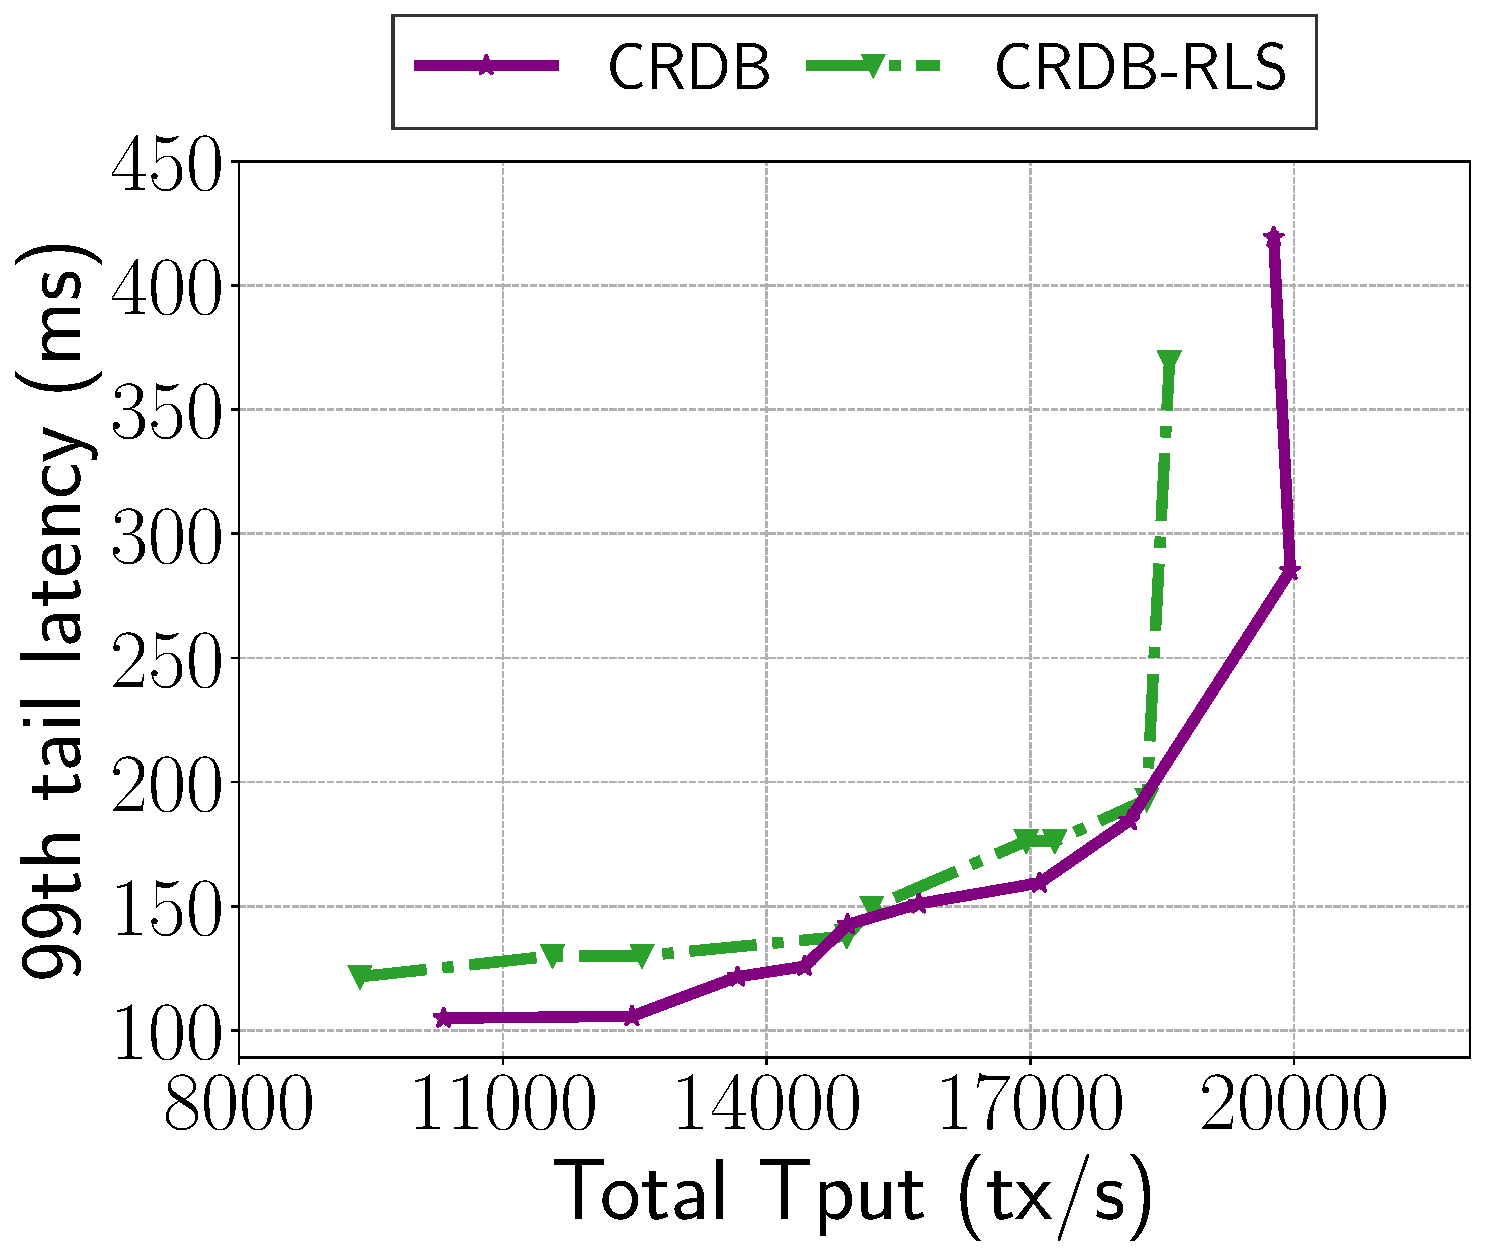
\includegraphics[width=0.49\columnwidth]{eval-figs/crdb-latency--tput-kv.pdf}
		\label{fig:eval:kv:overview}
	}
	\caption{Performance Comparison on Micro Workload.}\label{fig:eval:kv}
\end{figure}

\begin{figure}[t]
	\centering
	\subfloat[\footnotesize Throughput.]{
	   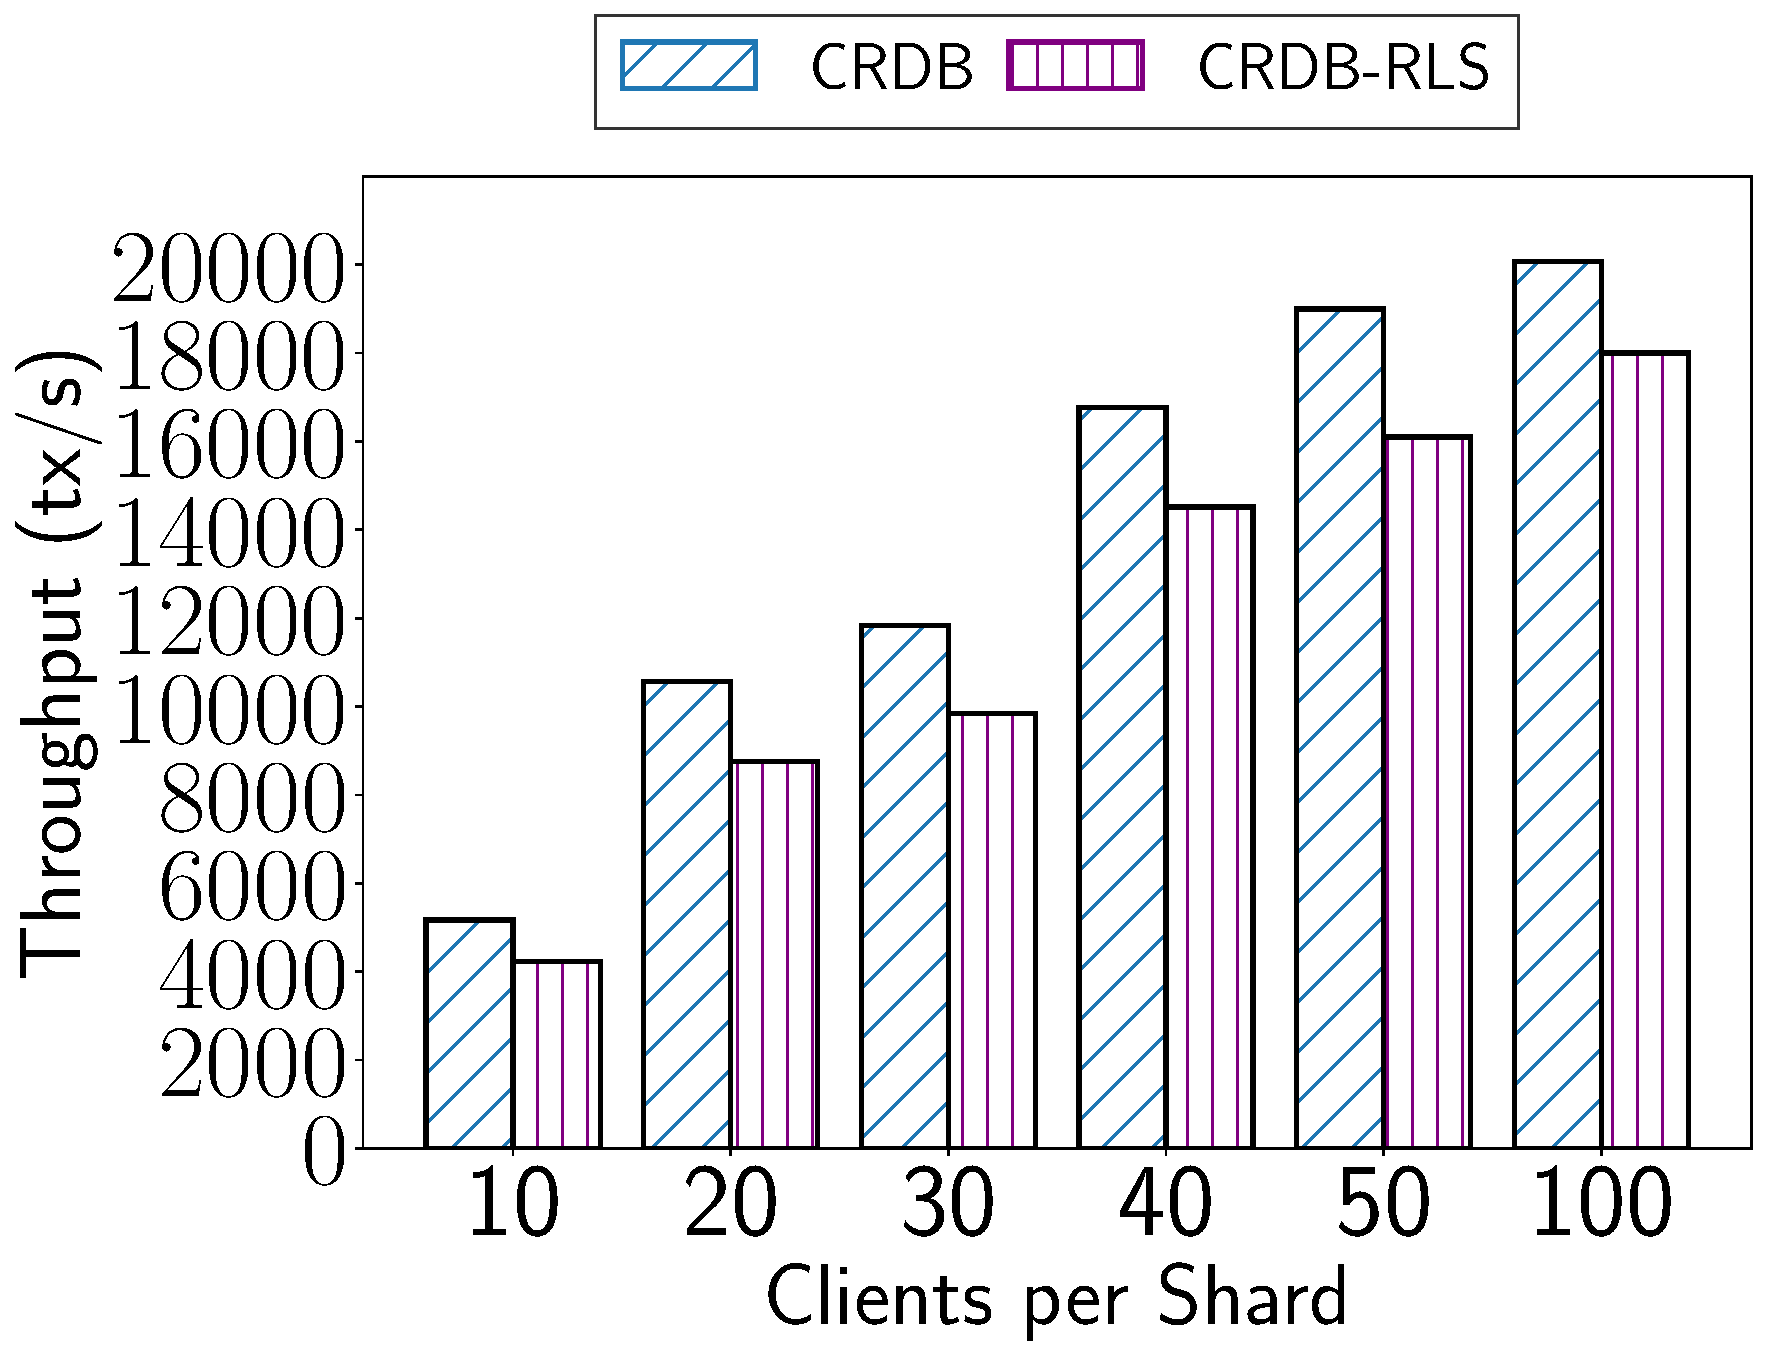
\includegraphics[width=0.49\columnwidth]{eval-figs/crdb-client--tput-ycsb.pdf}
	   \label{fig:crdb:eval:ycsb:throughput}
	}
	\subfloat[\footnotesize Overview.]{
		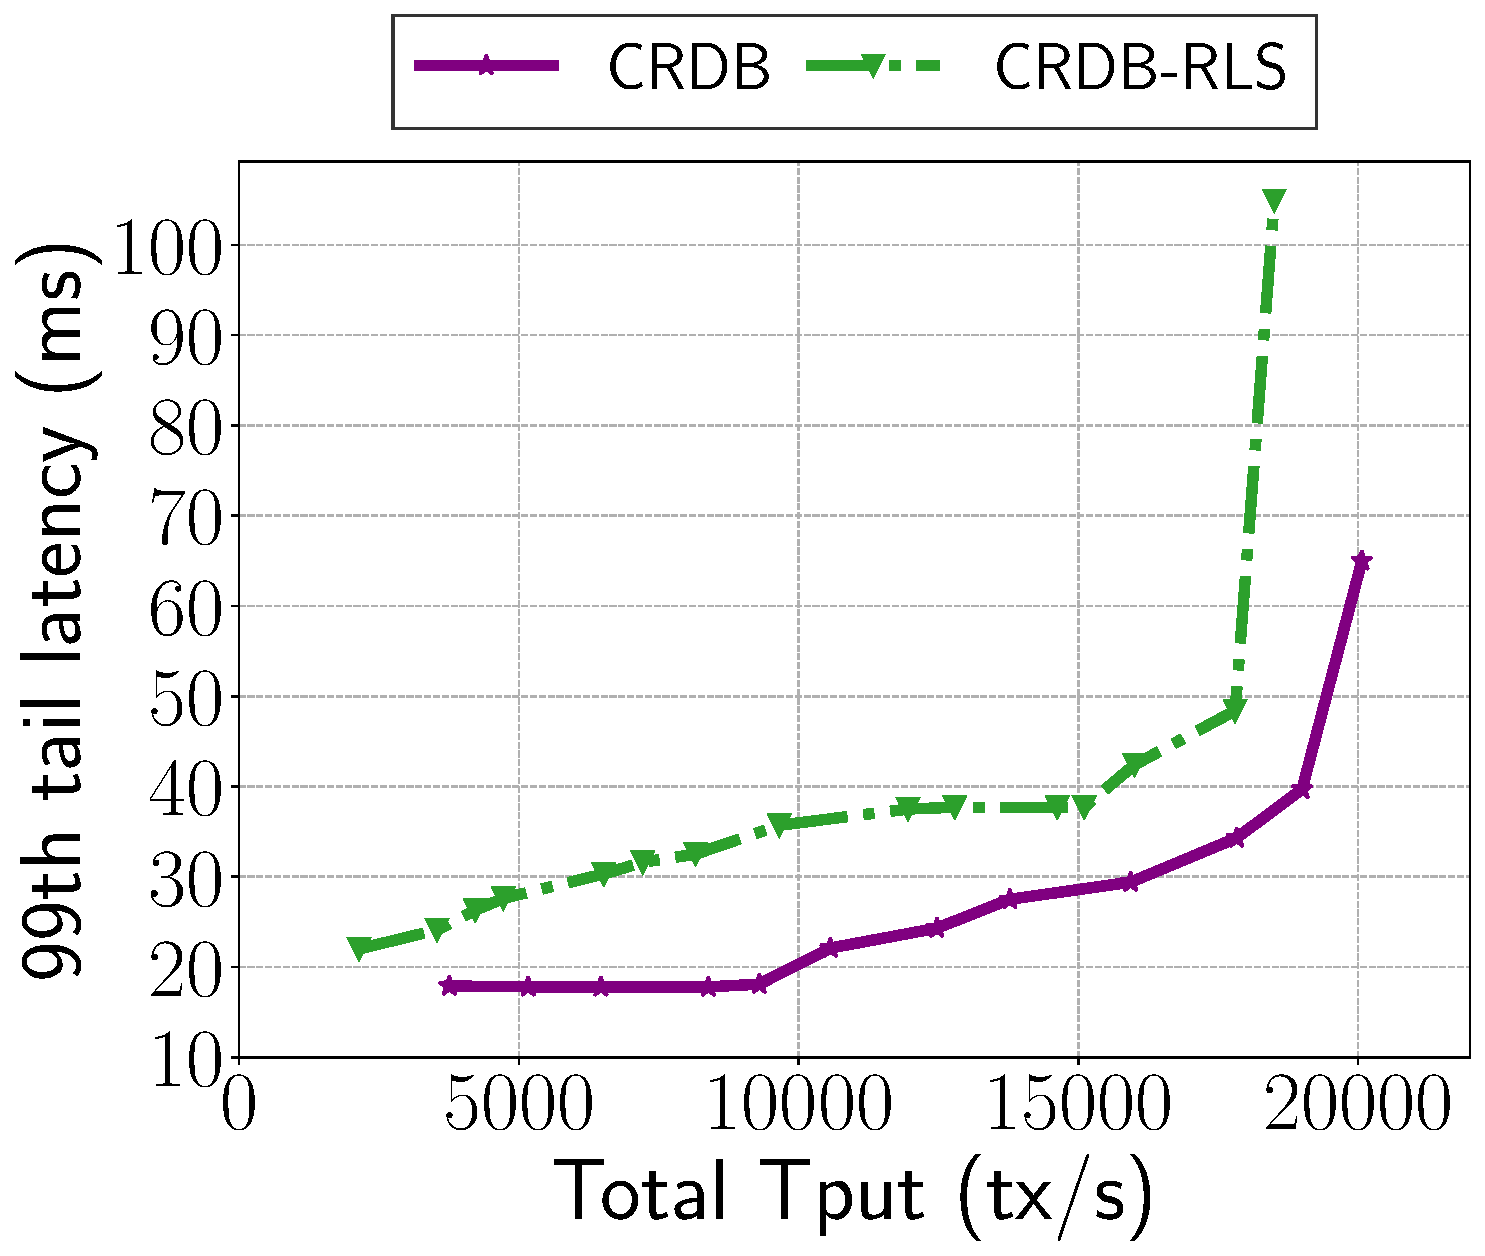
\includegraphics[width=0.49\columnwidth]{eval-figs/crdb-latency--tput-ycsb.pdf}
		\label{fig:crdb:eval:ycsb:overview}
	}
	\caption{Performance Comparison on YCSB-T (skewed).}\label{fig:crdb:eval:ycsb}
\end{figure}

Our observation of \crdbxx is that, to know whether a transaction $T_1$ may have finished before $T_2$ starts, instead of directly comparing the timestamps, a more intuitive method should be using active inquiry. In \crdb, transaction managers maintain the status of each transaction, and one can get the status of each transaction from the managers. Initially, \crdb does not adopt this active inquiry design because it can be inefficient and non-scalable to let all transactions contact a single node in a geo-distributed deployment. However, \xxcons's region-based approach enabled \crdb to record transaction states in a per-region manner (\algo{algo4}, Line 13) and enabled each transaction to inquire only relevant regions' managers (\algo{algo4}, Line 14), achieving both stronger consistency and high efficiency.

Like CRDB, CRDB-RLS allocates timestamps using hybrid-logical clocks (HLC), where physical time is
based on a node’s coarsely-synchronized system clock, and logical time is based on Lamport’s clocks. Such a mechanism benefits the design of CRDB-RLS as valid transactions can now adjust their timestamps based on logical time without frequently re-obtaining new timestamps.


\noindent\textbf{Implementations.} We implemented CRDB-RLS using the open-source codebase of CRDB with version v23.1.10 from the official sites. We modified the logic of obtaining a valid timestamp by recoding all used timestamps inside a region using sets. Our implementation is orthogonal to the optimizations introduced by its origin paper~\cite{taft2020cockroachdb} (e.g., write pipelining, parallel commits, and follower read). 

\subsection{Evaluation and Discussion} We used the same hardware and cluster setups as Spanner. For the deployments, we employed $10$ containers spanning uniformly over the machines, with each container running as a CRDB node. We used the multi-region SQL for Table partition and data replication.

\subsubsection{Performance on Micro Workload} As the configuration file of CRDB is complex and always critical to the performance, we calibrated our results by running the most basic built-in workloads provided by the CRDB codebase  (i.e., a transaction reads and writes to three keys spread uniformly across the cluster). The results are shown in \fig{fig:eval:kv}. The peak throughput of CRDB was $\sim20k$ tps, which aligns with the results shown on the official sites. Therefore, we believe our experimental results are representative. 

In addition to CRDB, we also test the performance of our implemented variation: CRDB-RLS. CRDB-RLS's peak throughput ($\sim18.6k$ tps) is slightly lower (7\%) than CRDB, while the latency is roughly the same. The slight performance degradation is caused by the higher cost of obtaining valid timestamps for IRTs.

\subsubsection{Performance on YCSB-T} We further compared the performance of CRDB and CRDB-RLS on the default YCSB-T (\chref{sec:spanner:eval}) using the calibrated configurations. The results are shown in \fig{fig:crdb:eval:ycsb}. Overall, CRDB-RLS achieved approximately $0.87\times$ to $0.91\times$ throughput compared to CRDB with various concurrencies. The peak throughput of CRDB-RLS was $12\%$ lower than CRDB, and the 99th tail latency of CRDB-RLS was $1.2\times$ to $1.6\times$ higher than CRDB.


CRDB-RLS incurred a more server performance drop on the skewed YCSB-T workloads. Compared to CRDB, CRDB-RLS may expand the contention footprint by involving more ongoing timestamps (i.e., line 16, Algorithm2). However, the overhead is still marginal, and the performance degradation is smaller than $\sim15\%$.





\subsection{Takeaways.} CRDB-RLS achieved similar performance as CRDB while providing strong consistency guarantees on real-time orders. This is because CRDB-RLS can efficiently capture ongoing transactions inside a region due to the fast networks. Recording ongoing transactions (known as transaction tables) is a common approach for processing transactions on a single machine or in a smaller cluster due to its simplicity and easy extension. We reused such an approach but with a more lightweight tracking method for ordering IRTs.